\documentclass{article} % For LaTeX2e
\usepackage{nips14submit_e,times}
\usepackage{amsmath}
\usepackage{amsthm}
\usepackage{amssymb}
\usepackage{mathtools}
\usepackage{hyperref}
\usepackage{url}
\usepackage{algorithm}
\usepackage[noend]{algpseudocode}
%\documentstyle[nips14submit_09,times,art10]{article} % For LaTeX 2.09

\usepackage{graphicx}
\usepackage{caption}
\usepackage{subcaption}

\def\eQb#1\eQe{\begin{eqnarray*}#1\end{eqnarray*}}
\def\eQnb#1\eQne{\begin{eqnarray}#1\end{eqnarray}}
\providecommand{\e}[1]{\ensuremath{\times 10^{#1}}}
\providecommand{\pb}[0]{\pagebreak}

\newcommand{\E}{\mathrm{E}}
\newcommand{\Var}{\mathrm{Var}}
\newcommand{\Cov}{\mathrm{Cov}}

\def\Qb#1\Qe{\begin{question}#1\end{question}}
\def\Sb#1\Se{\begin{solution}#1\end{solution}}

\newenvironment{claim}[1]{\par\noindent\underline{Claim:}\space#1}{}
\newtheoremstyle{quest}{\topsep}{\topsep}{}{}{\bfseries}{}{ }{\thmname{#1}\thmnote{ #3}.}
\theoremstyle{quest}
\newtheorem*{definition}{Definition}
\newtheorem*{theorem}{Theorem}
\newtheorem*{lemma}{Lemma}
\newtheorem*{question}{Question}
\newtheorem*{preposition}{Preposition}
\newtheorem*{exercise}{Exercise}
\newtheorem*{challengeproblem}{Challenge Problem}
\newtheorem*{solution}{Solution}
\newtheorem*{remark}{Remark}
\usepackage{verbatimbox}
\usepackage{listings}
\title{Probabilistic Method: \\
Problem Set I}


\author{
Youngduck Choi \\
CIMS \\
New York University\\
\texttt{yc1104@nyu.edu} \\
}


% The \author macro works with any number of authors. There are two commands
% used to separate the names and addresses of multiple authors: \And and \AND.
%
% Using \And between authors leaves it to \LaTeX{} to determine where to break
% the lines. Using \AND forces a linebreak at that point. So, if \LaTeX{}
% puts 3 of 4 authors names on the first line, and the last on the second
% line, try using \AND instead of \And before the third author name.

\newcommand{\fix}{\marginpar{FIX}}
\newcommand{\new}{\marginpar{NEW}}

\nipsfinalcopy % Uncomment for camera-ready version

\begin{document}


\maketitle

\begin{abstract}
This work contains solutions to the problem set I
of Probabilistic Method 2016 at Courant Institute of Mathematical Sciences.
\end{abstract}

\bigskip

\begin{question}[1]
\hfill
\begin{figure}[h!]
  \centering
    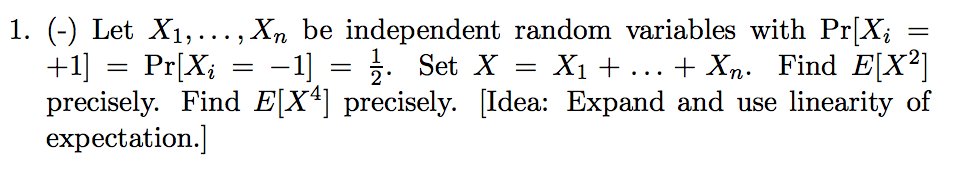
\includegraphics[width=1\textwidth]{PM-2-1.png}
\end{figure}
\end{question}
\begin{solution}
\end{solution}

\newpage

\begin{question}[2]
\hfill
\begin{figure}[h!]
  \centering
    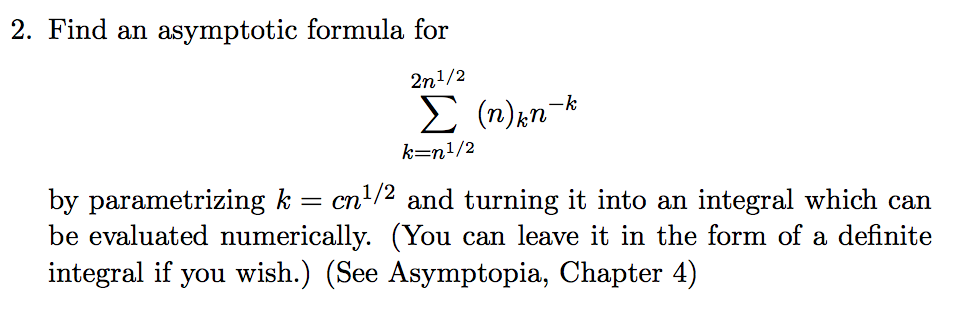
\includegraphics[width=1\textwidth]{PM-2-2.png}
\end{figure}
\end{question}
\begin{solution}

\end{solution}

\newpage

\begin{question}[3]
\hfill
\begin{figure}[h!]
  \centering
    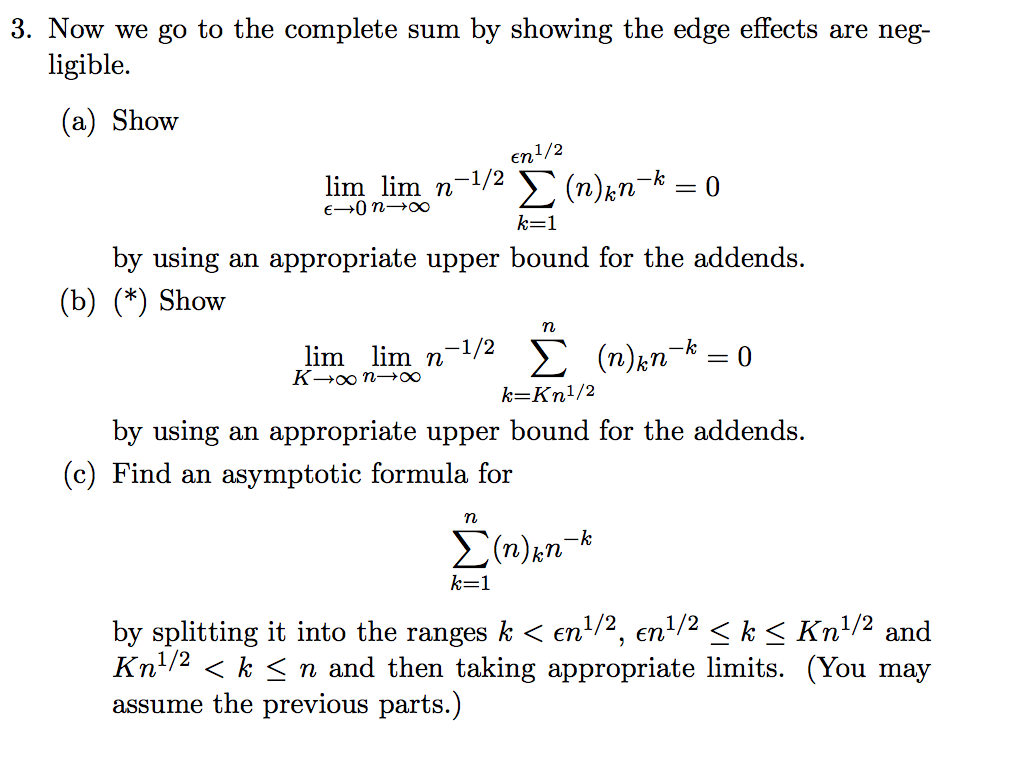
\includegraphics[width=1\textwidth]{PM-2-3.png}
\end{figure}
\end{question}
\begin{solution}
\end{solution}

\newpage

\begin{question}[4]
\hfill
\begin{figure}[h!]
  \centering
    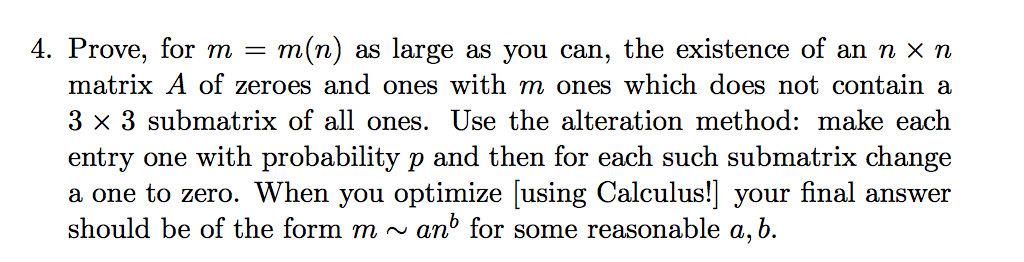
\includegraphics[width=1\textwidth]{PM-2-4.png}
\end{figure}
\end{question}
\begin{solution}
Consider a random $n \times n$ matrix, $M_{n}$, obtained 
by assigning each entry independently either $1$ or $0$, where the probability 
of assigning $1$ is $p$. Let $X$ be a random variable, which counts
number of $1$s in the matrix, and $Y$ be a random variable, which counts 
number of $3 \times 3$ submatrices of all $1$s. 
For any $3 \times 3$ submatrix $S$, let $Y_S$ be the
indicator random variable for the event for which the submatrix $S$ has entries of all $1$s,
so that $Y = \sum Y_{S}$. By Linearity of Expectation, we have
\eQb
E[Y] &=& \sum E[Y_S] = {n \choose 3}^2 p^{9}. \\
\eQe 
Clearly, $E[X] = n^2 p$. Therefore, again by Linearity of Expectation, it follows that
\eQb
E[X - Y] &=& n^2 p - {n \choose 3}^2 p^{9} = f(p). 
\eQe
Hence, there exists a random assignment, for which the number of $1$s minus 
the number of $3 \times 3$ submatrices of $1$ is at least $f(p)$.
Fix such a coloring. Select one entry from each submatrix and change to $0$. This leaves
the matrix with at least $f(p)$ entries with $1$. 

\smallskip

We now optimize this result by maximizing $f(p)$ with respect to $p$. Observe that $m$ 
is concave with respect to $p \in [0,1]$. Solving for the local maxima by setting the
first-order derivative equals to $0$, we get that $f$ is maximized at 
$p^* = (\dfrac{n^2}{9{n \choose 3}^2})^{\frac{1}{8}} = (\dfrac{2}{(n-1)(n-2)})^{\frac{1}{4}}$.
Substituting $p^*$ back into $f(p)$, we obtain
\eQb
f(p^*) &=& n^2(\dfrac{2}{(n-1)(n-2)})^{\frac{1}{4}} - {n \choose 3}^2 
\dfrac{n^2}{9 {n \choose 3}^2}(\dfrac{2}{(n-1)(n-2)})^{\frac{1}{4}} \\
&=& \dfrac{8}{9}n^2(\dfrac{2}{(n-1)(n-2)})^{\frac{1}{4}} \\ 
&\sim& \dfrac{8}{9}2^{\frac{1}{4}}n^{\frac{3}{2}}. 
\eQe
Recall that $m(n)$ be the minimum number of $1$ in $n \times n$ matrix, such that
there must exist a $3 \times 3$ submatrix of all $1$s.
We have shown that $m(n) = \Omega(n^{\frac{3}{2}})$.
\hfill $\qed$
\end{solution}

\newpage

\begin{question}[5]
\hfill
\begin{figure}[h!]
  \centering
    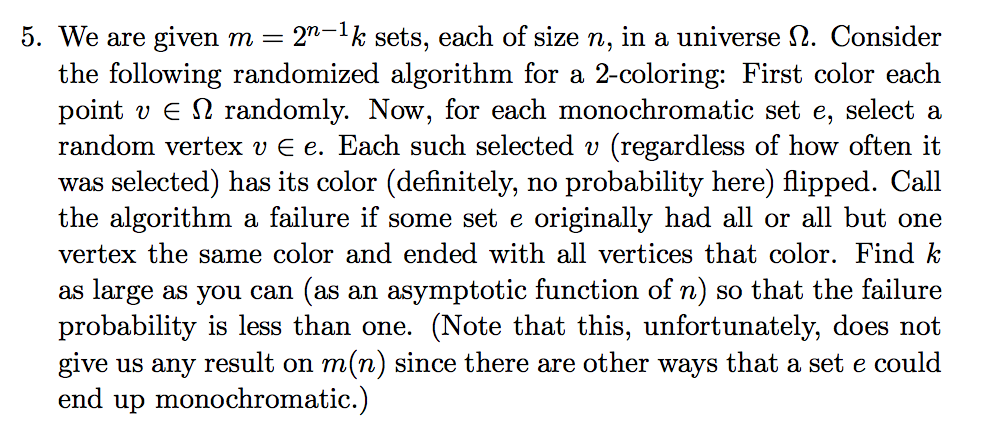
\includegraphics[width=1\textwidth]{PM-2-5.png}
\end{figure}
\end{question}
\begin{solution}
 
\end{solution}

\newpage

\begin{question}[6]
\hfill
\begin{figure}[h!]
  \centering
    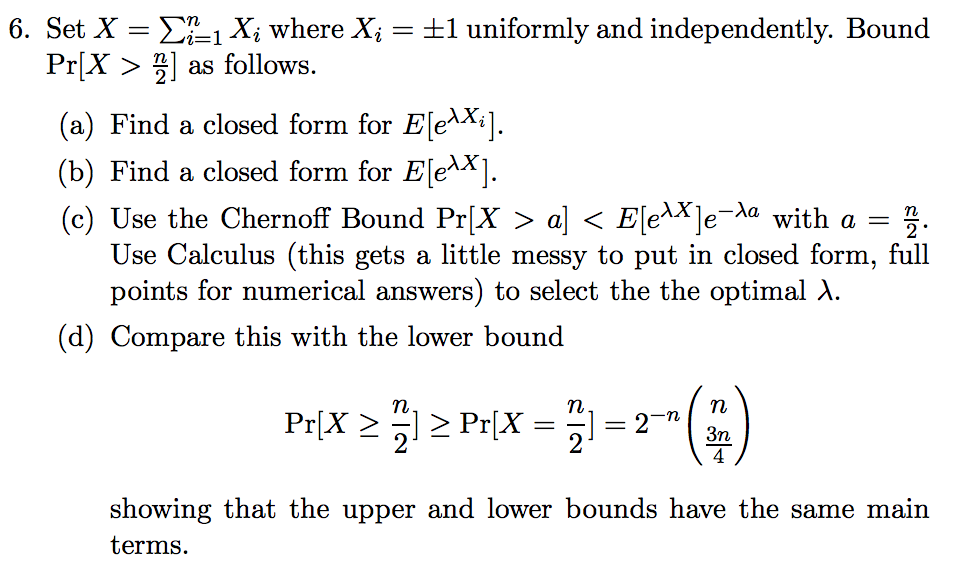
\includegraphics[width=1\textwidth]{PM-2-6.png}
\end{figure}
\end{question}
\begin{solution}
 
\end{solution}

\end{document}
